\documentclass[10pt,twocolumn,letterpaper]{article}

\usepackage{cvpr}
\usepackage{times}
\usepackage{epsfig}
\usepackage{graphicx}
\usepackage{amsmath}
\usepackage{amssymb}
\usepackage{subfigure}
\usepackage{algorithmic}
\usepackage{algorithm}
\renewcommand{\algorithmicrequire}{\textbf{Input:}}
\renewcommand{\algorithmicensure}{\textbf{Output:}}

% Include other packages here, before hyperref.

% If you comment hyperref and then uncomment it, you should delete
% egpaper.aux before re-running latex.  (Or just hit 'q' on the first latex
% run, let it finish, and you should be clear).
\usepackage[pagebackref=true,breaklinks=true,letterpaper=true,colorlinks,bookmarks=false]{hyperref}

\cvprfinalcopy % *** Uncomment this line for the final submission

\def\cvprPaperID{} % 
\def\httilde{\mbox{\tt\raisebox{-.5ex}{\symbol{126}}}}

% Pages are numbered in submission mode, and unnumbered in camera-ready
\ifcvprfinal\pagestyle{empty}\fi
\begin{document}

%%%%%%%%% TITLE
\title{ArcFace: Additive Angular Margin Loss for Deep Face Recognition}

\author{Jiankang Deng *\\
Imperial College London\\
{\tt\small j.deng16@imperial.ac.uk}
% For a paper whose authors are all at the same institution,
% omit the following lines up until the closing ``}''.
% Additional authors and addresses can be added with ``\and'',
% just like the second author.
% To save space, use either the email address or home page, not both
\and
Jia Guo \thanks{denotes equal contribution to this work.}\\
InsightFace\\
{\tt\small guojia@gmail.com}
\and
Niannan Xue\\
Imperial College London\\
{\tt\small n.xue15@imperial.ac.uk}
\and
Stefanos Zafeiriou\\
Imperial College London\\
{\tt\small s.zafeiriou@imperial.ac.uk}
}

\maketitle
%\thispagestyle{empty}

%%%%%%%%% ABSTRACT
\begin{abstract}
One of the main challenges in feature learning using Deep Convolutional Neural Networks (DCNNs) for large-scale face recognition is the design of appropriate loss functions that enhance discriminative power. Centre loss penalises the distance between the deep features and their corresponding class centres in the Euclidean space to achieve intra-class compactness. SphereFace assumes that the linear transformation matrix in the last fully connected layer can be used as a representation of the class centres in an angular space and penalises the angles between the deep features and their corresponding weights in a multiplicative way. Recently, a popular line of research is to incorporate margins in well-established loss functions in order to maximise face class separability. In this paper, we propose an Additive Angular Margin Loss (ArcFace) to obtain highly discriminative features for face recognition. The proposed ArcFace has a clear geometric interpretation due to the exact correspondence to the geodesic distance on the hypersphere. We present arguably the most extensive experimental evaluation of all the recent state-of-the-art face recognition methods on over 10 face recognition benchmarks including a new large-scale image database with trillion level of pairs and a large-scale video dataset. We show that ArcFace consistently outperforms the state-of-the-art and can be easily implemented with negligible computational overhead. We release all refined training data, training codes, pre-trained models and training logs\footnote{https://github.com/deepinsight/insightface}, which will help reproduce the results in this paper.
\end{abstract}

%%%%%%%%% BODY TEXT
\section{Introduction}

Face representation using Deep Convolutional Neural Network (DCNN) embedding is the method of choice for face recognition \cite{sun2014deep,taigman2014deepface,schroff2015facenet,parkhi2015deep}. DCNNs map the face image, typically after a pose normalisation step \cite{zhang2016joint}, into a feature that has small intra-class and large inter-class distance. 

\begin{figure}[t!]
\centering
\includegraphics[width=0.8\linewidth]{image/arcfaces.png}
\caption{Based on the centre \cite{liu2017sphereface} and feature \cite{tencent2017CosineFace} normalisation, all identities are distributed on a hypersphere. To enhance intra-class compactness and inter-class discrepancy, we consider four kinds of Geodesic Distance (GDis) constraint. (A) Margin-Loss: insert a geodesic distance margin between the sample and centres. (B) Intra-Loss: decrease the geodesic distance between the sample and the corresponding centre. (C) Inter-Loss: increase the geodesic distance between different centres. (D) Triplet-Loss: insert a geodesic distance margin between triplet samples. In this paper,  we propose an Additive Angular Margin Loss (ArcFace), which is exactly corresponded to the geodesic distance (Arc) margin penalty in (A), to enhance the discriminative power of face recognition model. Extensive experimental results show that the strategy of (A) is most effective. }
\vspace{-6mm}
\label{fig:arcfaceexplaination}
\end{figure}

There are two main lines of research to train DCNNs for face recognition. Those that train a multi-class classifier which can separate different identities in the training set, such by using a softmax classifier \cite{taigman2014deepface,parkhi2015deep,cao2017vggface2}, and those that learn directly an embedding, such as the triplet loss \cite{schroff2015facenet}. Based on the large-scale training data and the elaborate DCNN architectures, both the softmax-loss-based methods \cite{cao2017vggface2} and the triplet-loss-based methods \cite{schroff2015facenet} can obtain excellent performance on face recognition. However, both the softmax loss and the triplet loss have some drawbacks. For the softmax loss: (1) the size of the linear transformation matrix $W \in \mathbb{R}^{d \times n}$ increases linearly with the identities number $n$; (2) the learned features are separable for the closed-set classification problem but not discriminative enough for the open-set face recognition problem. For the triplet loss: (1) there is a combinatorial explosion in the number of face triplets especially for large-scale datasets, leading to a significant increase in the number of iteration steps; (2) semi-hard sample mining is a quite difficult problem for effective model training.

Several variants \cite{wen2016discriminative,deng2017marginal,zhang2016range,liu2017sphereface,tencent2017CosineFace,wang2018additive,chen2017noisy,wen2018rethinkingGM,qi2018facepami} have been proposed to enhance the discriminative power of the softmax loss. Wen \etal \cite{wen2016discriminative} pioneered the centre loss, the Euclidean distance between each feature vector and its class centre, to obtain intra-class compactness while the inter-class dispersion is guaranteed by the joint penalisation of the softmax loss. Nevertheless, updating the actual centres during training is extremely difficult as the number of face classes available for training has recently dramatically increased.

By observing that the weights from the last fully connected layer of a classification DCNN trained on the softmax loss bear conceptual similarities with the centres of each face class, the works in \cite{liu2017sphereface,liu2016large} proposed a multiplicative angular margin penalty to enforce extra intra-class compactness and inter-class discrepancy simultaneously, leading to a better discriminative power of the trained model. Even though Sphereface \cite{liu2017sphereface} introduced the important idea of angular margin, their loss function required a series of approximations in order to be computed, which resulted in an unstable training of the network. In order to stabilise training, they proposed a hybrid loss function which includes the standard softmax loss. Empirically, the softmax loss dominates the training process, because the integer-based multiplicative angular margin makes the target logit curve very precipitous and thus hinders convergence. CosFace \cite{tencent2017CosineFace,wang2018additive} directly adds cosine margin penalty to the target logit, which obtains better performance compared to SphereFace but admits much easier implementation and relieves the need for joint supervision from the softmax loss. 

In this paper, we propose an Additive Angular Margin Loss (ArcFace) to further improve the discriminative power of the face recognition model and to stabilise the training process. As illustrated in Figure \ref{fig:arcfacelossframework}, the dot product between the DCNN feature and the last fully connected layer is equal to the cosine distance after feature and weight normalisation. We utilise the arc-cosine function to calculate the angle between the current feature and the target weight. Afterwards, we add an additive angular margin to the target angle, and we get the target logit back again by the cosine function. Then, we re-scale all logits by a fixed feature norm, and the subsequent steps are exactly the same as in the softmax loss. The advantages of the proposed ArcFace can be summarised as follows:

\noindent{\bf Engaging.} ArcFace directly optimises the geodesic distance margin by virtue of the exact correspondence between the angle and arc in the normalised hypersphere. We intuitively illustrate what happens in the $512$-$D$ space via analysing the angle statistics between features and weights.

\noindent{\bf Effective.} ArcFace achieves state-of-the-art performance on ten face recognition benchmarks including large-scale image and video datasets. 

\noindent{\bf Easy.} ArcFace only needs several lines of code as given in Algorithm \ref{alg} and is extremely easy to implement in the computational-graph-based deep learning frameworks, \eg MxNet \cite{chen2015mxnet}, Pytorch \cite{paszke2017automatic} and Tensorflow \cite{abadi2016tensorflow}. Furthermore, contrary to the works in \cite{liu2017sphereface,liu2016large}, ArcFace does not need to be combined with other loss functions in order to have stable performance, 
and can easily converge on any training datasets.

\noindent{\bf Efficient.} ArcFace only adds negligible computational complexity during training. Current GPUs can easily support millions of identities for training and the model parallel strategy can easily support many more identities. 

\begin{figure*}[t!]
\centering
\includegraphics[width=0.9\linewidth]{image/arcfaceframework.png}
\vspace{-1mm}
\caption{Training a DCNN for face recognition supervised by the ArcFace loss. Based on the feature $x_i$ and weight $W$ normalisation, we get the $\cos\theta_j$ (logit) for each class as $W^T_j x_i$. We calculate the $arccos\theta_{y_i}$ and get the angle between the feature $x_i$ and the ground truth weight $W_{y_i}$. In fact, $W_j$ provides a kind of centre for each class. Then, we add an angular margin penalty $m$ on the target (ground truth) angle $\theta_{y_i}$. After that, we calculate $\cos(\theta_{y_i}+m)$ and multiply all logits by the feature scale $s$. The logits then go through the softmax function and contribute to the cross entropy loss.}
\vspace{-3mm}
\label{fig:arcfacelossframework}
\end{figure*}

\begin{algorithm*}[!htb]
\begin{algorithmic}
\STATE \textbf{Input:} Feature Scale $s$, Margin Parameter $m$ in Eq. \ref{eq:arcface}, Class Number $n$, Ground-Truth ID $gt$.
\vspace{-3mm}
\begin{enumerate} \setlength{\itemsep}{-\itemsep}
\item x = mx.symbol.L2Normalization (x, mode = 'instance')
\item W = mx.symbol.L2Normalization (W, mode = 'instance')
\item fc7 = mx.sym.FullyConnected (data = x, weight = W, no\_bias = True, num\_hidden = n)
\item original\_target\_logit = mx.sym.pick (fc7, gt, axis = 1)
\item theta = mx.sym.arccos (original\_target\_logit)
\item marginal\_target\_logit = mx.sym.cos (theta + m)
\item one\_hot = mx.sym.one\_hot (gt, depth = n, on\_value = 1.0, off\_value = 0.0)
\item fc7 = fc7 + mx.sym.broadcast\_mul (one\_hot, mx.sym.expand\_dims (marginal\_target\_logit - original\_target\_logit, 1))
\item fc7 = fc7 * s
\end{enumerate}
\vspace{-3mm}
\STATE \textbf{Output:} Class-wise affinity score $fc7$.
\end{algorithmic}
\caption{The Pseudo-code of ArcFace on MxNet}
\label{alg}
\end{algorithm*}

\section{Proposed Approach}

\subsection{ArcFace}

The most widely used classification loss function, softmax loss, is presented as follows:
\begin{equation}
L_1=-\frac{1}{N}\sum_{i=1}^{N}\log\frac{e^{W^T_{y_i} x_i+b_{y_i}}}{\sum_{j=1}^{n}e^{W^T_j x_i+b_j}},
\label{eq:softmax}
\vspace{-1mm}
\end{equation}
where $x_i\in\mathbb{R}^d$ denotes the deep feature of the $i$-th sample, belonging to the $y_i$-th class. The embedding feature dimension $d$ is set to $512$ in this paper following \cite{wen2016discriminative,zhang2016range,liu2017sphereface,tencent2017CosineFace}. $W_j\in\mathbb{R}^d$ denotes the $j$-th column of the weight $W \in \mathbb{R}^{d \times n}$ and $b_j\in\mathbb{R}^n $ is the bias term. The batch size and the class number are $N$ and $n$, respectively. Traditional softmax loss is widely used in deep face recognition \cite{parkhi2015deep,cao2017vggface2}. However, the softmax loss function does not explicitly optimise the feature embedding to enforce higher similarity for intra-class samples and diversity for inter-class samples, which results in a performance gap for deep face recognition under large intra-class appearance variations (\eg pose variations \cite{sengupta2016frontal,zheng2018cross} and age gaps \cite{Moschoglou2017AgeDB,zheng2017cross}) and large-scale test scenarios (\eg million \cite{kemelmacher2016megaface,whitelam2017iarpa,maze2018iarpa} or trillion pairs \cite{glintweb}).

For simplicity, we fix the bias $b_j=0$ as in \cite{liu2017sphereface}. Then, we transform the logit \cite{pereyra2017regularizing} as $W^T_j x_i=\left \| W_j \right \|\left \| x_i \right \|\cos\theta_j$, where $\theta_j$ is the angle between the weight $W_j$ and the feature $x_i$. Following \cite{liu2017sphereface,tencent2017CosineFace,wang2017normface}, we fix the individual weight $\left \| W_j \right \|=1$ by $l_2$ normalisation. Following \cite{ranjan2017l2,tencent2017CosineFace,wang2017normface,wang2018additive}, we also fix the embedding feature $\left \| x_i \right \|$ by $l_2$ normalisation and re-scale it to $s$.
The normalisation step on features and weights makes the predictions only depend on the angle between the feature and the weight. The learned embedding features are thus distributed on a hypersphere with a radius of $s$.
\begin{equation}
{L_2}=-\frac{1}{N}\sum_{i=1}^{N}\log\frac{e^{s\cos\theta_{y_i}}}{e^{s\cos\theta_{y_i}}+\sum_{j=1,j\neq  y_i}^{n}e^{s\cos\theta_{j}}}.
\label{eq:l2featweight}
\vspace{-1mm}
\end{equation}

As the embedding features are distributed around each feature centre on the hypersphere, we add an additive angular margin penalty $m$ between $x_i$ and $W_{y_i}$ to simultaneously enhance the intra-class compactness and inter-class discrepancy. Since the proposed additive angular margin penalty is equal to the geodesic distance margin penalty in the normalised hypersphere, we name our method as ArcFace. 
\begin{equation}
{L_3}=-\frac{1}{N}\sum_{i=1}^{N}\log\frac{e^{s(\cos(\theta_{y_i}+m))}}{e^{s(\cos(\theta_{y_i}+m))}+\sum_{j=1,j\neq  y_i}^{n}e^{s\cos\theta_{j}}}.
\label{eq:arcface}
\vspace{-1mm}
\end{equation}

We select face images from 8 different identities containing enough samples (around 1,500 images/class) to train 2-D feature embedding networks with the softmax and ArcFace loss, respectively. As illustrated in Figure \ref{fig:compactness}, the softmax loss provides roughly separable feature embedding but produces noticeable ambiguity in decision boundaries, while the proposed ArcFace loss can obviously enforce a more evident gap between the nearest classes. 

\begin{figure}[h!]
\centering
\subfigure[Softmax]{
\label{fig:compactnesssoftmaxnorm}
\includegraphics[width=0.18\textwidth]{image/compactness/softmaxnorm.pdf}}
\subfigure[ArcFace]{
\label{fig:compactnessarcfacenorm}
\includegraphics[width=0.18\textwidth]{image/compactness/arcfacenorm.pdf}}
\caption{Toy examples under the softmax and ArcFace loss on 8 identities with 2D features. Dots indicate samples and lines refer to the centre direction of each identity. Based on the feature normalisation, all face features are pushed to the arc space with a fixed radius. The geodesic distance gap between closest classes becomes evident as the additive angular margin penalty is incorporated.}
\vspace{-6mm}
\label{fig:compactness}
\end{figure}

\subsection{Comparison with SphereFace and CosFace}

\noindent{\bf Numerical Similarity.} In SphereFace \cite{liu2017sphereface,liu2016large}, ArcFace, and CosFace \cite{tencent2017CosineFace,wang2018additive}, three different kinds of margin penalty are proposed, \eg multiplicative angular margin $m_1$, additive angular margin $m_2$, and additive cosine margin $m_3$, respectively. From the view of numerical analysis, different margin penalties, no matter add on the angle \cite{liu2017sphereface} or cosine space \cite{tencent2017CosineFace}, all enforce the intra-class compactness and inter-class diversity by penalising the target logit \cite{pereyra2017regularizing}. In Figure \ref{fig:soatargetlogit}, we plot the target logit curves of SphereFace, ArcFace and CosFace under their best margin settings. We only show these target logit curves within $[20^{\circ}, 100^{\circ}]$ because the angles between $W_{y_i}$ and $x_i$ start from around $90^{\circ}$ (random initialisation) and end at around $30^{\circ}$ during ArcFace training as shown in Figure \ref{fig:thetadistribution}. Intuitively, there are three factors in the target logit curves that affect the performance, \ie the starting point, the end point and the slope. 

\begin{figure}[h!]
\centering
\subfigure[$\theta_j$ Distributions]{
\label{fig:thetadistribution}
\includegraphics[width=0.23\textwidth]{image/targetlogit/arcFacehiststartend.pdf}}
\subfigure[Target Logits Curves]{
\label{fig:soatargetlogit}
\includegraphics[width=0.23\textwidth]{image/targetlogit/TargetLogitCurve.pdf}}
\caption{Target logit analysis. (a) $\theta_j$ distributions from start to end during ArcFace training. (2) Target logit curves for softmax, SphereFace, ArcFace, CosFace and combined margin penalty ($\cos(m_1 \theta+m_2)-m_3$).}
\vspace{-4mm}
\label{fig:targetlogitscurves}
\end{figure}

By combining all of the margin penalties, we implement SphereFace, ArcFace and CosFace in an united framework with $m_1$, $m_2$ and $m_3$ as the hyper-parameters. 
\begin{equation}
\small
{L_4}=-\frac{1}{N}\sum_{i=1}^{N}\log\frac{e^{s(\cos(m_1\theta_{y_i}+m_2)-m_3)}}{e^{s(\cos(m_1\theta_{y_i}+m_2)-m_3)}+\sum_{j=1,j\neq  y_i}^{n}e^{s\cos\theta_{j}}}.
\label{eq:combineloss}
\vspace{-1mm}
\end{equation}
As shown in Figure \ref{fig:soatargetlogit}, by combining all of the above-motioned margins ($\cos(m_1 \theta+m_2)-m_3$), we can easily get some other target logit curves which also have high performance. 

\noindent{\bf Geometric Difference.} Despite the numerical similarity between ArcFace and previous works, the proposed additive angular margin has a better geometric attribute as the angular margin has the exact correspondence to the geodesic distance. As illustrated in Figure \ref{fig:binarymargin}, we compare the decision boundaries under the binary classification case. The proposed ArcFace has a constant linear angular margin throughout the whole interval. By contrast, SphereFace and CosFace only have a nonlinear angular margin. 

\begin{figure}[h!]
\centering
\includegraphics[width=1\linewidth]{image/difference/margincompare.png}
\caption{Decision margins of different loss functions under binary classification case. The dashed line represents the decision boundary, and the grey areas are the decision margins.}
\vspace{-4mm}
\label{fig:binarymargin}
\end{figure}

The minor difference in margin designs can have ``butterfly effect'' on the model training. For example, the original SphereFace \cite{liu2017sphereface} employs an annealing optimisation strategy. To avoid divergence at the beginning of training, joint supervision from softmax is used in SphereFace to weaken the multiplicative margin penalty. We implement a new version of SphereFace without the integer requirement on the margin by employing the arc-cosine function instead of using the complex double angle formula. In our implementation, we find that $m=1.35$ can obtain similar performance compared to the original SphereFace without any convergence difficulty. 

\subsection{Comparison with Other Losses}

Other loss functions can be designed based on the angular representation of features and weight-vectors. For examples, we can design a loss to enforce intra-class compactness and inter-class discrepancy on the hypersphere. As shown in Figure \ref{fig:arcfaceexplaination}, we compare with three other losses in this paper. 

\noindent{\bf Intra-Loss} is designed to improve the intra-class compactness by decreasing the angle/arc between the sample and the ground truth centre.
\begin{equation}
L_5=L_2 + \frac{1}{\pi N} \sum_{i=1}^{N} \theta_{y_i}.
\label{eq:intraloss}
\vspace{-1mm}
\end{equation}

\noindent{\bf Inter-Loss} targets at enhancing inter-class discrepancy by increasing the angle/arc between different centres. 
\begin{equation}
L_6=L_2 - \frac{1}{\pi N \left ( n -1\right )}  \sum_{i=1}^{N}  \sum_{j=1,j\neq y_i}^{n} \arccos(W^T_{y_i}W_j).
\label{eq:interloss}
\vspace{-1mm}
\end{equation}
The Inter-Loss here is a special case of the Minimum Hyper-spherical Energy (MHE) method \cite{liu2018learning}. In \cite{liu2018learning}, both hidden layers and output layers are regularised by MHE. In the MHE paper, a special case of loss function was also proposed by combining the SphereFace loss with MHE loss on the last layer of the network. 

\noindent{\bf Triplet-loss} aims at enlarging the angle/arc margin between triplet samples. In FaceNet \cite{schroff2015facenet}, Euclidean margin is applied on the normalised features. Here, we employ the triplet-loss by the angular representation of our features as $\arccos({x_{i}^{pos} x_{i}}) + m \leq \arccos({x_i^{neg} x_{i}})$. 

\section{Experiments}

\subsection{Implementation Details}

\noindent {\bf Datasets.} As given in Table \ref{table:dataset}, we separately employ CASIA \cite{yi2014learning}, VGGFace2 \cite{cao2017vggface2}, MS1MV2 and DeepGlint-Face (including MS1M-DeepGlint and Asian-DeepGlint) \cite{glintweb} as our training data in order to conduct fair comparison with other methods. Please note that the proposed MS1MV2 is a semi-automatic refined version of the MS-Celeb-1M dataset \cite{guo2016ms}. To best of our knowledge, we are the first to employ ethnicity-specific annotators for large-scale face image annotations, as the boundary cases (\eg hard samples and noisy samples) are very hard to distinguish if the annotator is not familiar with the identity. During training, we explore efficient face verification datasets (\eg LFW \cite{huang2007labeled}, CFP-FP \cite{sengupta2016frontal}, AgeDB-30 \cite{Moschoglou2017AgeDB}) to check the improvement from different settings. Besides the most widely used LFW \cite{huang2007labeled} and YTF \cite{wolf2011face} datasets, we also report the performance of ArcFace on the recent large-pose and large-age datasets(\eg CPLFW \cite{zheng2018cross} and CALFW \cite{zheng2017cross}). We also extensively test the proposed ArcFace on large-scale image datasets (\eg MegaFace \cite{kemelmacher2016megaface}, IJB-B \cite{whitelam2017iarpa}, IJB-C \cite{maze2018iarpa} and Trillion-Pairs \cite{glintweb}) and video datasets (iQIYI-VID \cite{IQIYI2018}).

\begin{table}[t!]
\begin{center}
\begin{tabular}{c|c|c}
\hline
 Datasets   & \#Identity & \#Image/Video\\
\hline
CASIA \cite{yi2014learning} & 10K  & 0.5M  \\
% CelebA  \cite{liu2015deep}       & 10.2K  & 0.2M  \\
% VGGFace1 \cite{parkhi2015deep}   & 2.6K & 0.98M  \\
VGGFace2 \cite{cao2017vggface2}     & 9.1K & 3.3M  \\
% UMDFace  \cite{bansal2017umdfaces}  & 8.3K & 0.37M  \\
% Starnow-ArcFace                  & 8.3K & 0.37M  \\
% MS1M      \cite{guo2016ms}       & 100K & 10M \\
% MS1M-IBUG \cite{deng2017marginal}& 85K  & 3.8M \\
MS1MV2                             & 85K  & 5.8M \\   
MS1M-DeepGlint \cite{glintweb}   & 87K  & 3.9M \\
Asian-DeepGlint \cite{glintweb}     & 94 K  & 2.83M\\
% IQIYI-train \cite{IQIYI2018}    & 4,934  & 219,677\\
% \hline
% Validation Dataset   & Identity Num & Image Num\\
\hline
LFW \cite{huang2007labeled}   & 5,749  & 13,233 \\
CFP-FP \cite{sengupta2016frontal} & 500 & 7,000\\
AgeDB-30 \cite{Moschoglou2017AgeDB} & 568 & 16,488 \\
CPLFW \cite{zheng2018cross} & 5,749  & 11,652 \\
CALFW \cite{zheng2017cross} & 5,749  & 12,174 \\
YTF   \cite{wolf2011face} & 1,595  & 3,425 \\ 
\hline
MegaFace \cite{kemelmacher2016megaface} & 530 (P) & 1M (G) \\
IJB-B    \cite{whitelam2017iarpa}       & 1,845   & 76.8K \\
IJB-C    \cite{maze2018iarpa}           & 3,531   & 148.8K \\
Trillion-Pairs \cite{glintweb}          & 5,749 (P) & 1.58M (G)\\
iQIYI-VID \cite{IQIYI2018}              & 4,934   & 172,835\\
% IQIYI-val \cite{IQIYI2018}    & 4,934  & 172,860\\
% Image Test   & Gallery  Identity Num & Distractors Num\\
% \hline\hline
% IJB-B    \cite{whitelam2017iarpa}       & 1, 845  & - \\
% IJB-C    \cite{maze2018iarpa}           & 3, 531   & - \\
% MegaFace-FaceScrub \cite{kemelmacher2016megaface} & 530  & 1M \\
% TrillionPairs \cite{glintweb}           & 5.7K  & 1.58M \\
% \hline
% Video Test   &     Identity Num & Video Num\\
% \hline\hline
% YTF   \cite{wolf2011face} & 1,595  & 3,425 \\ 
% iQIYI-VID \cite{IQIYI2018}    & 4,934  & 172,835\\
%  565,372, of which training set 219,677, validation set 172,860, test set 172,835
\hline
\end{tabular}
\end{center}
\caption{Face datasets for training and testing. ``(P)'' and ``(G)'' refer to the probe and gallery set, respectively.}
\label{table:dataset}
\vspace{-4mm}
\end{table}


\noindent {\bf Experimental Settings.} For data prepossessing, we follow the recent papers \cite{liu2017sphereface,tencent2017CosineFace} to generate the normalised face crops ($112\times112$) by utilising five facial points. For the embedding network, we employ the widely used CNN architectures, ResNet50 and ResNet100 \cite{he2016deep,han2016deep}. After the last convolutional layer, we explore the BN \cite{ioffe2015batch}-Dropout \cite{srivastava2014dropout}-FC-BN structure to get the final $512$-$D$ embedding feature. 
In this paper, we use ([training dataset, network structure, loss]) to facilitate understanding of the experimental settings. 

We follow \cite{tencent2017CosineFace} to set the feature scale $s$ to 64 and choose the angular margin $m$ of ArcFace at $0.5$. All experiments in this paper are implemented by MXNet \cite{chen2015mxnet}. We set the batch size to $512$ and train models on four NVIDIA Tesla P40 (24GB) GPUs. On CASIA, the learning rate starts from $0.1$ and is divided by $10$ at 20K, 28K iterations. The training process is finished at 32K iterations. On MS1MV2, we divide the learning rate at 100K,160K iterations and finish at 180K iterations. We set momentum to $0.9$ and weight decay to $5e-4$. During testing, we only keep the feature embedding network without the fully connected layer (160MB for ResNet50 and 250MB for ResNet100) and extract the $512$-$D$ features ($8.9$ ms/face for ResNet50 and $15.4$ ms/face for ResNet100) for each normalised face. To get the embedding features for templates (\eg IJB-B and IJB-C) or videos (\eg YTF and iQIYI-VID), we simply calculate the feature centre of all images from the template or all frames from the video. Note that, overlap identities between the training set and the test set are removed for strict evaluations, and we only use a single crop for all testing. 
% Due to space limitation, all details regarding the networks used for all the experiments are provided in the supplementary materials. 

\subsection{Ablation Study on Losses}

In Table \ref{table:losscompare}, we first explore the angular margin setting for ArcFace on the CASIA dataset with ResNet50. The best margin observed in our experiments was $0.5$. Using the proposed combined margin framework in Eq. \ref{eq:combineloss}, it is easier to set the margin of SphereFace and CosFace which we found to have optimal performance when setting at $1.35$ and $0.35$, respectively.  
Our implementations for both SphereFace and CosFace can lead to excellent performance without observing any difficulty in convergence. The proposed ArcFace achieves the highest verification accuracy on all three test sets. 
In addition, we performed extensive experiments with the combined margin framework (some of the best performance was observed for CM1 (1, 0.3, 0.2) and CM2 (0.9, 0.4, 0.15)) guided by the target logit curves in Figure \ref{fig:soatargetlogit}.  The combined margin framework led to better performance than individual SphereFace and CosFace but upper-bounded by the performance of ArcFace. 

Besides the comparison with margin-based methods, we conduct a further comparison between ArcFace and other losses which aim at enforcing intra-class compactness (Eq. \ref{eq:intraloss}) and inter-class discrepancy (Eq. \ref{eq:interloss}). As the baseline we have chosen the softmax loss and we have observed performance drop on CFP-FP and AgeDB-30 after weight and feature normalisation. By combining the softmax with the intra-class loss, the performance improves on CFP-FP and AgeDB-30. However, combining the softmax with the inter-class loss only slightly improves the accuracy. The fact that Triplet-loss outperforms Norm-Softmax loss indicates the importance of margin in improving the performance. However, employing margin penalty within triplet samples is less effective than inserting margin between samples and centres as in ArcFace. Finally, we incorporate the Intra-loss, Inter-loss and Triplet-loss into ArcFace, but no improvement is observed, which leads us to believe that ArcFace is already enforcing intra-class compactness, inter-class discrepancy and classification margin.

\begin{table}[ht!]
\begin{center}
\begin{tabular}{c|c|c|c}
\hline
Loss Functions   & LFW & CFP-FP & AgeDB-30 \\
\hline
ArcFace (0.4)         & 99.53 & 95.41 & 94.98   \\
ArcFace (0.45)        & 99.46 & 95.47 & 94.93 \\
ArcFace (0.5)         & {\bf 99.53} & {\bf 95.56} & {\bf 95.15}\\
ArcFace (0.55)        & 99.41  & 95.32   & 95.05   \\
\hline
SphereFace \cite{liu2017sphereface}  & 99.42 & - & - \\
SphereFace (1.35)                    & 99.11 & 94.38 & 91.70 \\
CosFace \cite{tencent2017CosineFace} & 99.33 & - & - \\
CosFace (0.35)                       & 99.51 & 95.44 & 94.56 \\
\hline
CM1 (1, 0.3, 0.2)                    & 99.48 & 95.12 & 94.38 \\
CM2 (0.9, 0.4, 0.15)                 & 99.50 & 95.24 & 94.86 \\
\hline
Softmax              & 99.08 & 94.39 & 92.33 \\
Norm-Softmax (NS)    & 98.56 & 89.79 & 88.72 \\
NS+Intra             & 98.75 & 93.81 & 90.92 \\
NS+Inter             & 98.68 & 90.67 & 89.50 \\
NS+Intra+Inter       & 98.73 & 94.00 & 91.41 \\
Triplet (0.35)       & 98.98 & 91.90 & 89.98 \\
ArcFace+Intra        & 99.45 & 95.37 & 94.73 \\
ArcFace+Inter        & 99.43 & 95.25 & 94.55 \\
ArcFace+Intra+Inter  & 99.43 & 95.42 & 95.10 \\
ArcFace+Triplet      & 99.50 & 95.51 & 94.40  \\
\hline
\end{tabular}
\end{center}
\vspace{-2mm}
\caption{Verification results ($\%$) of different loss functions ([CASIA, ResNet50, loss*]).}
\label{table:losscompare}
\vspace{-3mm}
\end{table}

To get a better understanding of ArcFace's superiority, we give the detailed angle statistics on training data (CASIA) and test data (LFW) under different losses in Table \ref{table:angledistributionchanges2}. We find that (1) $W_j$ is nearly synchronised with embedding feature centre for ArcFace ($14.29^{\circ}$), but there is an obvious deviation ($44.26^{\circ}$) between $W_j$ and the embedding feature centre for Norm-Softmax. Therefore, the angles between $W_j$ cannot absolutely represent the inter-class discrepancy on training data. Alternatively, the embedding feature centres calculated by the trained network are more representative. (2) Intra-Loss can effectively compress intra-class variations but also brings in smaller inter-class angles. (3) Inter-Loss can slightly increase inter-class discrepancy on both $W$ (directly) and the embedding network (indirectly), but also raises intra-class angles. (4) ArcFace already has very good intra-class compactness and inter-class discrepancy. (5) Triplet-Loss has similar intra-class compactness but inferior inter-class discrepancy compared to ArcFace. In addition, ArcFace has a more distinct margin than Triplet-Loss on the test set as illustrated in Figure \ref{fig:losshist}.

\begin{table}[t!]
\begin{center}
\begin{tabular}{c|c|c|c|c|c}
\hline
       & NS  & ArcFace & IntraL & InterL & TripletL\\
\hline
W-EC   &44.26&14.29& 8.83& 46.85 & - \\
W-Inter&69.66&71.61&31.34& 75.66 & - \\
Intra1 &50.50&38.45&17.50& 52.74 & 41.19 \\
Inter1 &59.23&65.83&24.07& 62.40 & 50.23 \\
\hline
Intra2 &33.97&28.05&12.94& 35.38 & 27.42 \\
Inter2 &65.60&66.55&26.28& 67.90 & 55.94\\
\hline
\end{tabular}
\end{center}
\caption{The angle statistics under different losses ([CASIA, ResNet50, loss*]). Each column denotes one particular loss. ``W-EC'' refers to the mean of angles between $W_j$ and the corresponding embedding feature centre. ``W-Inter'' refers to the mean of minimum angles between $W_j$'s. ``Intra1'' and ``Intra2'' refer to the mean of angles between $x_i$ and the embedding feature centre on CASIA and LFW, respectively. ``Inter1'' and ``Inter2'' refer to the mean of minimum angles between embedding feature centres on CASIA and LFW, respectively.}
\label{table:angledistributionchanges2}
\vspace{-4mm}
\end{table}


\begin{figure}[h!]
\centering
\subfigure[ArcFace]{
\label{fig:arc}
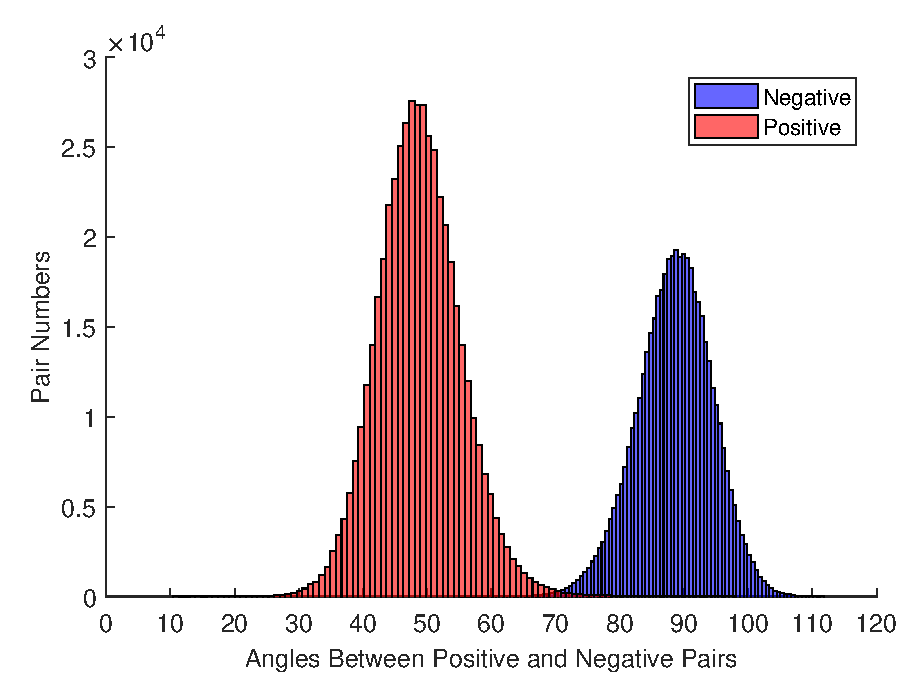
\includegraphics[width=0.2\textwidth]{image/lossdiff/t_arc.pdf}}
\subfigure[Triplet-Loss]{
\label{fig:triplet}
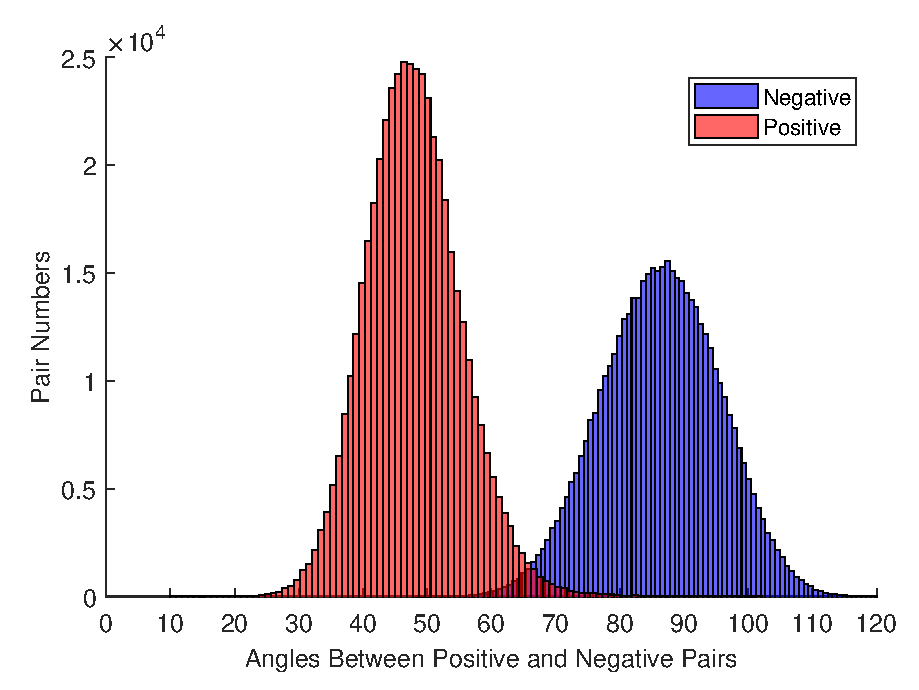
\includegraphics[width=0.2\textwidth]{image/lossdiff/t_triplet.pdf}}
\caption{Angle distributions of all positive pairs and random negative pairs ($\sim0.5$M) from LFW. Red area indicates positive pairs while blue indicates negative pairs. All angles are represented in degree. ([CASIA, ResNet50, loss*]).}
\vspace{-2mm}
\label{fig:losshist}
\end{figure}


\subsection{Evaluation Results}

\noindent {\bf Results on LFW, YTF, CALFW and CPLFW.}
LFW \cite{huang2007labeled} and YTF \cite{wolf2011face} datasets are the most widely used benchmark for unconstrained face verification on images and videos. In this paper, we follow the \textit{unrestricted with labelled outside data} protocol to report the performance. As reported in Table \ref{table:lfwytf}, ArcFace trained on MS1MV2 with ResNet100 beats the baselines (\eg SphereFace \cite{liu2017sphereface} and CosFace \cite{tencent2017CosineFace}) by a significant margin on both LFW and YTF, which shows that the additive angular margin penalty can notably enhance the discriminative power of deeply learned features, demonstrating the effectiveness of ArcFace.

\begin{table}[t!]
\begin{center}
\begin{tabular}{c|c|c|c}
\hline
Method &  \#Image &  LFW       & YTF\\
\hline
% SphereFace \cite{liu2017sphereface}      &99.42        &95.0    \\
% SphereFace+ \cite{liu2018learning}       &99.47        &-       \\
% CosFace \cite{tencent2017CosineFace}     &99.33        &{\bf 96.1}    \\
% CASIA, R50, ArcFace                      &{\bf 99.533} &95.24   \\
% \hline\hline
DeepID \cite{sun2014deep}            & 0.2M    &99.47 &93.20\\
Deep Face \cite{taigman2014deepface} & 4.4M    &97.35 &91.4\\
VGG Face \cite{parkhi2015deep}       &2.6M     &98.95 &97.30\\
FaceNet \cite{schroff2015facenet}    & 200M    &99.63 &95.10\\
Baidu \cite{liu2015targeting}     &1.3M       &99.13 & -\\
Center Loss \cite{wen2016discriminative} & 0.7M &99.28 &94.9\\
Range Loss \cite{zhang2016range}     &5M    &99.52 &93.70\\
Marginal Loss \cite{deng2017marginal} & 3.8M   &99.48 &95.98 \\
SphereFace \cite{liu2017sphereface}  & 0.5M     &99.42 &95.0\\
SphereFace+ \cite{liu2018learning}   & 0.5M    &99.47 & - \\
CosFace \cite{tencent2017CosineFace} & 5M    &99.73 &97.6\\
MS1MV2, R100, ArcFace               & 5.8M   &{\bf 99.83} & {\bf 98.02} \\
\hline
\end{tabular}
\end{center}
\vspace{-2mm}
\caption{Verification performance ($\%$) of different methods on LFW and YTF.}
\label{table:lfwytf}
\vspace{-4mm}
\end{table}

Besides on LFW and YTF datasets, we also report the performance of ArcFace on the recently introduced datasets (\eg CPLFW \cite{zheng2018cross} and CALFW \cite{zheng2017cross}) which show higher pose and age variations with same identities from LFW. Among all of the open-sourced face recognition models, the ArcFace model is evaluated as the top-ranked face recognition model as shown in Table \ref{table:calfwandcplfw}, outperforming counterparts by an obvious margin. In Figure \ref{fig:histgramsall}, we illustrate the angle distributions (predicted by ArcFace model trained on MS1MV2 with ResNet100) of both positive and negative pairs on LFW, CFP-FP, AgeDB-30, YTF, CPLFW and CALFW. We can clearly find that the intra-variance due to pose and age gaps significantly increases the angles between positive pairs thus making the best threshold for face verification increasing and generating more confusion regions on the histogram. 

\begin{table}[t!]
\begin{center}
\begin{tabular}{c|c|c|c}
\hline
Method                                  & LFW & CALFW & CPLFW\\
\hline
HUMAN-Individual                        & 97.27 & 82.32 & 81.21 \\
HUMAN-Fusion                            & 99.85 & 86.50 & 85.24 \\
\hline
Center Loss \cite{wen2016discriminative}&98.75 & 85.48 & 77.48  \\
SphereFace \cite{liu2017sphereface}     &99.27 & 90.30 & 81.40  \\
VGGFace2  \cite{cao2017vggface2}        &99.43 & 90.57 & 84.00   \\
% ArcFace                               &{\bf 99.82} & {\bf 95.45} & {\bf 86.60} \\
MS1MV2, R100, ArcFace                   &{\bf 99.82} & {\bf 95.45} & {\bf 92.08} \\
\hline
\end{tabular}
\end{center}
\vspace{-2mm}
\caption{Verification performance ($\%$) of open-sourced face recognition models on LFW, CALFW and CPLFW.}
\label{table:calfwandcplfw}
\vspace{-4mm}
\end{table}

\begin{figure}[h!]
\centering
\subfigure[LFW ($99.83\%$)]{
\label{fig:lfwhist}
\includegraphics[width=0.15\textwidth]{figure/validation/arcfacehist/lfw-arcface.pdf}}
\subfigure[CFP-FP ($98.37\%$)]{
\label{fig:cfpfp}
\includegraphics[width=0.15\textwidth]{figure/validation/arcfacehist/cfp-fp-arcface.pdf}}
\subfigure[AgeDB ($98.15\%$)]{
\label{fig:cfpfp}
\includegraphics[width=0.15\textwidth]{figure/validation/arcfacehist/agedb-30-arcface.pdf}}
\subfigure[YTF ($98.02\%$)]{
\label{fig:cfpfp}
\includegraphics[width=0.15\textwidth]{figure/validation/arcfacehist/YTF-arcface.pdf}}
\subfigure[CPLFW ($92.08\%$)]{
\label{fig:cfpfp}
\includegraphics[width=0.15\textwidth]{figure/validation/arcfacehist/cplfw-arcface.pdf}}
\subfigure[CALFW ($95.45\%$)]{
\label{fig:cfpfp}
\includegraphics[width=0.15\textwidth]{figure/validation/arcfacehist/calfw-arcface.pdf}}
\caption{Angle distributions of both positive and negative pairs on LFW, CFP-FP, AgeDB-30, YTF, CPLFW and CALFW. Red area indicates positive pairs while blue indicates negative pairs. All angles are represented in degree. ([MS1MV2, ResNet100, ArcFace])}
% \vspace{-6mm}
\label{fig:histgramsall}
\end{figure}

\noindent {\bf Results on MegaFace.} The MegaFace dataset \cite{kemelmacher2016megaface} includes 1M images of 690K different individuals  as the gallery set and 100K photos of $530$ unique individuals from FaceScrub \cite{ng2014data} as the probe set. On MegaFace, there are two testing scenarios (identification and verification) under two protocols (large or small training set). The training set is defined as large if it contains more than 0.5M images. For the fair comparison, we train ArcFace on CAISA and MS1MV2 under the small protocol and large protocol, respectively. In Table \ref{table:megaface}, ArcFace trained on CASIA achieves the best single-model identification and verification performance, not only surpassing the strong baselines (\eg SphereFace \cite{liu2017sphereface} and CosFace \cite{tencent2017CosineFace}) but also outperforming other published methods \cite{wen2016discriminative,liu2018learning}.  

As we observed an obvious performance gap between identification and verification, we performed a thorough manual check in the whole MegaFace dataset and found many face images with wrong labels, which significantly affects the performance. Therefore, we manually refined the whole MegaFace dataset and report the correct performance of ArcFace on MegaFace. On the refined MegaFace, ArcFace still clearly outperforms CosFace and achieves the best performance on both verification and identification.

Under large protocol, ArcFace surpasses FaceNet \cite{schroff2015facenet} by a clear margin and obtains comparable results on identification and better results on verification compared to CosFace \cite{tencent2017CosineFace}. Since CosFace employs a private training data, we retrain CosFace on our MS1MV2 dataset with ResNet100. Under fair comparison, ArcFace shows superiority over CosFace  and forms an upper envelope of CosFace under both identification and verification scenarios as shown in Figure \ref{fig:megafacecmcroc}.

\begin{table}[t!]
\begin{center}
\begin{tabular}{c|c|c}
\hline
Methods  & Id ($\%$) & Ver ($\%$) \\
\hline
Softmax  \cite{liu2017sphereface}                      & 54.85 & 65.92 \\
Contrastive Loss\cite{liu2017sphereface,sun2014deep}   & 65.21 & 78.86\\
Triplet \cite{liu2017sphereface,schroff2015facenet}    & 64.79 & 78.32\\
Center Loss\cite{wen2016discriminative}                & 65.49 & 80.14 \\
SphereFace \cite{liu2017sphereface} & 72.729 & 85.561  \\
% SphereFace+FeatNorm \cite{liu2017sphereface} & 75.42 & 88.32  \\
% SphereFace(Ensemble) \cite{liu2017sphereface} & 75.766& -  \\
CosFace \cite{tencent2017CosineFace} & 77.11 & 89.88 \\
AM-Softmax \cite{wang2018additive}   & 72.47 & 84.44 \\
% CosFace(Ensemble) \cite{tencent2017CosineFace} & 79.54 & - \\
SphereFace+ \cite{liu2018learning}   & 73.03 & - \\
\hline
CASIA, R50, ArcFace                  & 77.50 & 92.34\\
CASIA, R50, ArcFace, R               & 91.75 & 93.69\\
% CASIA, R50, CosFace, R                & todo & todo\\
\hline\hline
FaceNet \cite{schroff2015facenet}    & 70.49       & 86.47 \\
CosFace \cite{tencent2017CosineFace} & 82.72       & 96.65 \\
\hline
MS1MV2, R100, ArcFace               & 81.03       & 96.98 \\
MS1MV2, R100, CosFace               & 80.56       & 96.56  \\
MS1MV2, R100, ArcFace, R            & 98.35       & 98.48 \\
MS1MV2, R100, CosFace, R            & 97.91       & 97.91  \\
\hline
\end{tabular}
\end{center}
\vspace{-2mm}
\caption{Face identification and verification evaluation of different methods on MegaFace Challenge1 using FaceScrub as the probe set. ``Id'' refers to the rank-1 face identification accuracy with 1M distractors, and ``Ver'' refers to the face verification TAR at $10^{-6}$ FAR. ``R'' refers to data refinement on both probe set and 1M distractors. ArcFace obtains state-of-the-art performance under both small and large protocols.}
\label{table:megaface}
\vspace{-4mm}
\end{table}

\begin{figure}[h!]
\centering
\subfigure[CMC]{
\label{fig:megafacecmc}
\includegraphics[width=0.228\textwidth]{figure/megaface/facescrubCMC.pdf}}
\subfigure[ROC]{
\label{fig:megafaceroc}
\includegraphics[width=0.228\textwidth]{figure/megaface/facescrubROC.pdf}}
\caption{CMC and ROC curves of different models on MegaFace. Results are evaluated on both original and refined MegaFace dataset.}
\vspace{-3mm}
\label{fig:megafacecmcroc}
\end{figure}

\noindent {\bf Results on IJB-B and IJB-C.} The IJB-B dataset \cite{whitelam2017iarpa} contains $1,845$ subjects with $21.8$K still images and $55$K frames from $7,011$ videos. In total, there are $12,115$ templates with $10,270$ genuine matches and $8$M impostor matches. The IJB-C dataset \cite{whitelam2017iarpa} is a further extension of IJB-B, having $3,531$ subjects with $31.3$K still images and $117.5$K frames from $11,779$ videos. In total, there are $23,124$ templates with $19,557$ genuine matches and $15,639$K impostor matches. 

On the IJB-B and IJB-C datasets, we employ the VGG2 dataset as the training data and the ResNet50 as the embedding network to train ArcFace for the fair comparison with the most recent methods \cite{cao2017vggface2,xie2018multicolumn,xie2018comparator}.
In Table \ref{tab:ijb}, we compare the TAR (@FAR=1e-4) of ArcFace with the previous state-of-the-art models \cite{cao2017vggface2,xie2018multicolumn,xie2018comparator}. ArcFace can obviously boost the performance on both IJB-B and IJB-C (about $3\sim5\%$, which is a significant reduction in the error). Drawing support from more training data (MS1MV2) and deeper neural network (ResNet100), ArcFace can further improve the TAR (@FAR=1e-4) to $94.2\%$ and $95.6\%$ on IJB-B and IJB-C, respectively.
In Figure \ref{pic:ijb}, we show the full ROC curves of the proposed ArcFace on IJB-B and IJB-C \footnote{https://github.com/deepinsight/insightface/tree/master/Evaluation/IJB}, and ArcFace achieves impressive performance even at FAR=1e-6 setting a new baseline. 

\begin{table}[t!]
\begin{center}
\begin{tabular}{c|c|c}
\hline
Method           & IJB-B & IJB-C  \\ 
\hline
ResNet50 \cite{cao2017vggface2} &0.784 & 0.825\\
SENet50 \cite{cao2017vggface2}  &0.800 & 0.840\\
ResNet50+SENet50 \cite{cao2017vggface2}&0.800& 0.841\\
MN-v \cite{xie2018multicolumn}&0.818 & 0.852\\
MN-vc \cite{xie2018multicolumn}&0.831 & 0.862\\
ResNet50+DCN(Kpts) \cite{xie2018comparator}&0.850 & 0.867\\
ResNet50+DCN(Divs) \cite{xie2018comparator}&0.841 & 0.880\\
SENet50+DCN(Kpts)  \cite{xie2018comparator}&0.846 & 0.874\\
SENet50+DCN(Divs)  \cite{xie2018comparator}&0.849 & 0.885\\
\hline
VGG2, R50, ArcFace    & 0.898 & 0.921\\
MS1MV2, R100, ArcFace & {\bf 0.942} & {\bf 0.956}\\
\hline
\end{tabular}
\end{center}
\vspace{-2mm}
\caption{1:1 verification TAR (@FAR=1e-4) on the IJB-B and IJB-C dataset.}
\vspace{-4mm}
\label{tab:ijb}
\end{table}

\begin{figure}[h!]
\centering
\subfigure[ROC for IJB-B]{
\label{pic:ijbb_roc} 
\includegraphics[width=0.226\textwidth]{figure/test/IJB/ijbb_compare.pdf}
}
\subfigure[ROC for IJB-C]{
\label{pic:ijbc_roc} 
\includegraphics[width=0.226\textwidth]{figure/test/IJB/ijbc_compare.pdf}
}
\caption{ROC curves of 1:1 verification protocol on the IJB-B and IJB-C dataset.}
\vspace{-2mm}
\label{pic:ijb}
\end{figure}

\noindent {\bf Results on Trillion-Pairs.} The Trillion-Pairs dataset \cite{glintweb} provides 1.58M images from Flickr as the gallery set and 274K images from 5.7k LFW \cite{huang2007labeled} identities as the probe set. Every pair between gallery and probe set is used for evaluation (0.4 trillion pairs in total). In Table \ref{table:trillionpairs}, we compare the performance of ArcFace trained on different datasets. The proposed MS1MV2 dataset obviously boosts the performance compared to CASIA and even slightly outperforms the DeepGlint-Face dataset, which has a double identity number. When combining all identities from MS1MV2 and Asian celebrities from DeepGlint, ArcFace achieves the best identification performance $84.840\%$ (@FPR=1e-3) and comparable verification performance compared to the most recent submission (CIGIT\_IRSEC) from the lead-board.  

\begin{table}[t!]
\begin{center}
\begin{tabular}{c|c|c}
\hline
Method      & Id (@FPR=1e-3)    & Ver(@FPR=1e-9) \\
\hline
CASIA        & 26.643      & 21.452\\
%VGG2,R50   & 42.838      & 41.438\\
MS1MV2       & 80.968      & 78.600\\
DeepGlint-Face    & 80.331      & 78.586\\
% MS1MV2+Asian & 83.928      & 80.315\\
MS1MV2+Asian  & {\bf 84.840} (1st)  & 80.540\\
\hline
CIGIT\_IRSEC   & 84.234 (2nd) & {\bf 81.558} (1st) \\
\hline
\end{tabular}
\end{center}
\vspace{-2mm}
\caption{Identification and verification results ($\%$) on the Trillion-Pairs dataset. ([Dataset*, ResNet100, ArcFace])}
\label{table:trillionpairs}
\vspace{-2mm}
\end{table}

\noindent {\bf Results on iQIYI-VID.} The iQIYI-VID challenge \cite{IQIYI2018} contains 565,372 video clips (training set 219,677, validation set 172,860, and test set 172,835) of 4934 identities from iQIYI variety shows, films and television dramas. The length of each video ranges from $1$ to $30$ seconds. This dataset supplies multi-modal cues, including face, cloth, voice, gait and subtitles, for character identification. The iQIYI-VID dataset employs MAP@100 as the evaluation indicator. MAP (Mean Average Precision) refers to the overall average accuracy rate, which is the mean of the average accuracy rate of the corresponding videos of person ID retrieved in the test set for each person ID (as the query) in the training set.

As shown in Table \ref{table:iqiyivid}, ArcFace trained on combined MS1MV2 and Asian datasets with ResNet100 sets a high baseline (MAP=($79.80\%$)). Based on the embedding feature for each training video, we train an additional three-layer fully connected network with a classification loss to get the customised feature descriptor on the iQIYI-VID dataset. The MLP learned on the iQIYI-VID training set significantly boosts the MAP by $6.60\%$. Drawing support from the model ensemble and context features from the off-the-shelf object and scene classifier \cite{mxnetmodels}, our final result surpasses the runner-up by a clear margin ( $0.99\%$). 

\begin{table}[t!]
\begin{center}
\begin{tabular}{c|c}
\hline
Method                 & MAP($\%$) \\
\hline
MS1MV2+Asian, R100, ArcFace &  79.80    \\
+ MLP                  &  86.40    \\
+ Ensemble             &  88.26    \\
+ Context     &  {\bf 88.65 (1st)} \\
\hline
Other Participant       & 87.66 (2nd) \\
\hline
\end{tabular}
\end{center}
\vspace{-2mm}
\caption{MAP of our method on the iQIYI-VID test set. ``MLP'' refers to a three-layer fully connected network trained on the iQIYI-VID training data. }
\label{table:iqiyivid}
\vspace{-6mm}
\end{table}

\section{Conclusions}

In this paper, we proposed an Additive Angular Margin Loss function, which can effectively enhance the discriminative power of feature embeddings learned via DCNNs for face recognition. In the most comprehensive experiments reported in the literature we demonstrate that our method consistently outperforms the state-of-the-art. Code and details have been released under the MIT license.

\section{Appendix}

\subsection{Parallel Acceleration}

{\bf Can we apply ArcFace on large-scale identities?} Yes, millions of identities are not a problem.

The concept of Centre ($W$) is indispensable in ArcFace, but the parameter size of Centre ($W$) is proportional to the number of classes. When there are millions of identities in the training data, the proposed ArcFace confronts with substantial training difficulties, \eg excessive GPU memory consumption and massive computational cost, even at a prohibitive level.

In our implementation \footnote{https://github.com/deepinsight/insightface/tree/master/recognition}, we employ a parallel acceleration strategy \cite{debingzhang} to relieve this problem. We optimise our training code to easily and efficiently support {\bf million} level identities on a single machine by parallel acceleration on both feature $x$ (it known as the general data parallel strategy) and centre $W$ (we named it as the centre parallel strategy). As shown in Figure \ref{fig:parallel}, our parallel acceleration on both feature $x$ and centre $W$ can significantly decrease the GPU memory consumption and accelerate the training speed. Even for one million identities trained on 8*1080ti (11GB), our implementation (ResNet 50, batch size 8*64, feature dimension 512 and float point 32) can still run at 800 samples per second. Compared to the approximate acceleration method proposed in \cite{zhang2018accelerated}, our implementation has no performance drop.

\begin{figure}[h!]
\small
\centering
\subfigure[GPU Memory]{
\label{fig:memory}
\includegraphics[width=0.4\textwidth]{parallel/memory.pdf}}
\subfigure[Training Speed]{
\label{fig:speed}
\includegraphics[width=0.4\textwidth]{parallel/speed.pdf}}
\caption{Parallel acceleration on both feature $x$ and centre $W$. Setting: ResNet 50, batch size 8*64, feature dimension 512, float point 32, GPU 8*P40 (24GB).}
\label{fig:parallel}
\end{figure}

In Figure \ref{fig:parallelillus}, we illustrate the main calculation steps of the parallel acceleration by simple matrix partition, which can be easily grasped and reproduced by beginners \cite{c231n}.

(1) Get feature ($x$). Face embedding features are aggregated into one feature matrix (batch size 8*64 $\times$ feature dimension 512) from 8 GPU cards. The size of the aggregated feature matrix is only 1MB, and the communication cost is negligible when we transfer the feature matrix. 

(2) Get similarity score matrix ($score=xW$). We copy the feature matrix into each GPU, and concurrently multiply the feature matrix by the centre sub-matrix (feature dimension 512 $\times$ identity number 1M/8) to get the similarity score sub-matrix (batch size 512 $\times$ identity number 1M/8) on each GPU. The similarity score matrix goes forward to calculate the ArcFace loss and the gradient. Here, we conduct a simple matrix partition on the centre matrix and the similarity score matrix along the identity dimension, and there is no communication cost on the centre and similarity score matrix. Both the centre sub-matrix and the similarity score sub-matrix are only 256MB on each GPU. 

(3) Get gradient on centre ($dW$). We transpose the feature matrix on each GPU, and concurrently multiply the transposed feature matrix by the gradient sub-matrix of the similarity score. 

(4) Get gradient on feature ($x$). We concurrently multiply the gradient sub-matrix of similarity score by the transposed centre sub-matrix and sum up the outputs from 8 GPU cards to get the gradient on feature $x$. 

Considering the communication cost (MB level), our implementation of ArcFace can be easily and efficiently trained on millions of identities by clusters.

% \vspace{-10pt}
\begin{figure}[h!]
\small
\centering
\subfigure[$x$]{
\label{fig:s1}
\includegraphics[width=0.48\textwidth]{parallel/S1.png}}
\subfigure[$score=xW$]{
\label{fig:s2}
\includegraphics[width=0.48\textwidth]{parallel/S2.png}}
\subfigure[$dW=x^T dscore$]{
\label{fig:s3}
\includegraphics[width=0.48\textwidth]{parallel/S3.png}}
\subfigure[$dx=dscore W^T$]{
\label{fig:s4}
\includegraphics[width=0.48\textwidth]{parallel/S4.png}}
\caption{Parallel calculation by simple matrix partition. Setting: ResNet 50, batch size 8*64, feature dimension 512, float point 32, identity number 1 Million, GPU 8 * 1080ti (11GB). {\bf Communication cost: 1MB (feature $x$). Training speed: 800 samples/second}.}
\label{fig:parallelillus}
\vspace{-10pt}
\end{figure}

\subsection{Feature Space Analysis}

{\bf Is the $512$-d hypersphere space large enough to hold large-scale identities?} Theoretically, Yes. 

We assume that the identity centre $W_j$'s follow a realistically spherical uniform distribution, the expectation of the nearest neighbour separation\cite{Brauchart18} is
\begin{equation}
\small
\mathbb{E}[\theta(W_j)]\rightarrow n^{-\frac{2}{d-1}}\Gamma(1+\frac{1}{d-1})(\frac{\Gamma(\frac{d}{2})}{2\sqrt{\pi}(d-1)\Gamma(\frac{d-1}{2})})^{-\frac{1}{d-1}},
\label{eq:largespace}
\end{equation}
where $d$ is the space dimension, $n$ is the identity number, and $\theta(W_j)=\min_{1\leq i,j\leq n, i\ne j}\arccos(W_i,W_j)\forall i,j$. In Figure \ref{fig:largespace}, we give $\mathbb{E}[\theta(W_j)]$ in the $128$-d, $256$-d and $512$-d space with the class number ranging from $10K$ to $100M$. The high-dimensional space is so large that $\mathbb{E}[\theta(W_j)]$ decreases slowly when the class number increases exponentially. 
% However, $W_j$'s does not exactly follow a realistically spherical uniform distribution for face recognition. 

\begin{figure}[ht!]
\centering
\includegraphics[width=0.4\textwidth]{image/largespace/minangledecrease.pdf}
\caption{The high-dimensional space is so large that the mean of the nearest angles decreases slowly when the class number increases exponentially.}
\vspace{-4mm}
\label{fig:largespace}
\end{figure}



{\small
\bibliographystyle{ieee}
\bibliography{egbib}
}

\end{document}
